\section{Durchführung}
\label{sec:Durchführung}

\subsection{Messung des Entladevorgangs}
Die Zeitkonstante $RC$ wird durch die Messung des Entladevorgangs des Kondensators bestimmt. 
Mit der in Abb. \ref{fig:4a} dargestellten Schaltung wird die am Kondensator gemessene Spannung $U_{C}(t)$ auf einem
Oszilloskop in Abhängigkeit von der Zeit $t$ angezeigt. Dabei muss darauf geachtet werden, dass sich die Spannung 
$U_{C}(t)$ innerhalb des Aufzeichnungszeitraums um den Faktor $5$ bis $10$ ändert. Sobald eine geeignete Kurve auf dem 
Bildschirm zu erkennen ist, werden mindestens $10$ Messwertpaare aufgenommen.
\begin{figure}
  \centering
  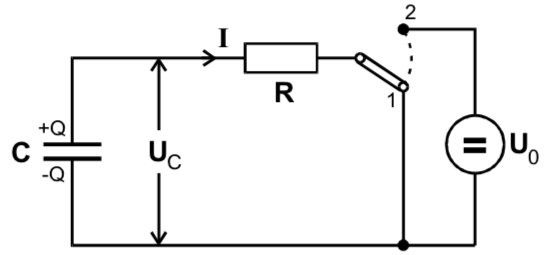
\includegraphics[width= 8cm, height=5cm]{build/4a.png}
  \caption{Schaltung zur Bestimmung der Zeitkonstanten eines RC-Gliedes durch den Entladevorgang des Kondensators.}
  \label{fig:4a}
\end{figure}

\subsection{Messung der Amplitude der Kondensatorspannung}
Mittels der Schaltung, die in Abb. \ref{fig:4b} dargestellt wird, wird die Amplitude der Kondensatorspannung in 
Abängigkeit von der Frequenz gemessen. Es werden $15$ Wertepaare aufgenommen.
Die Amplitude wird dabei in Abhängigkeit von der Frequenz über drei Zehnerpotenzenmhinweg gemessen.
\begin{figure}
  \centering
  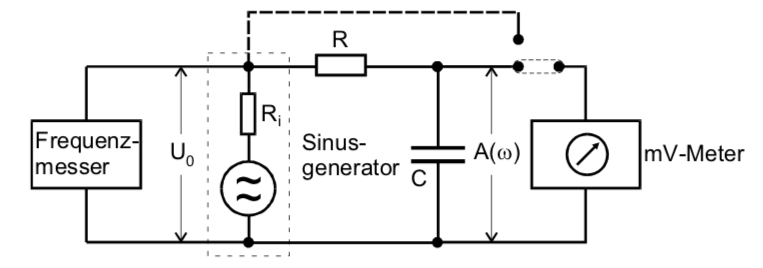
\includegraphics[width=10cm, height=5cm]{build/4b.png}
  \caption{Schaltung zur Bestimmung der Zeitkonstanten eines RC-Gliedes durch die Amplitude der Kondensatorspannung.}
  \label{fig:4b}
\end{figure}

\subsection{Messung der Phasenverschiebung}
Zur Ermittlung der Phasenverschiebung werden, wie in Abb. \ref{fig:4c} dargestellt, die Kondensatorspannung $U_{C}(t)$ 
und die Generatorspannung $U_{G}(t)$ an ein Zweistrahl-Oszilloskop angeschlossen. Dabei wird der Abstand $a$ der 
Nulldurchgänge der beiden Kurven gemessen. Die Periodendauer $T$ ergibt sich aus der eingestellten Frequenz.%geteilt um auf den Winkel $\phi$ der Phasenverschiebung zu kommen. 
\begin{figure}
  \centering
  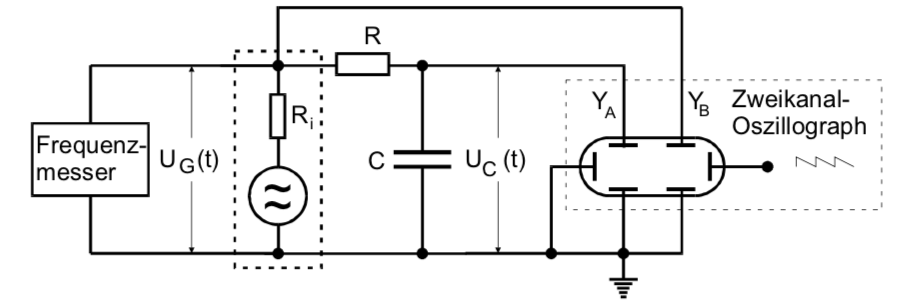
\includegraphics[width= 10cm, height=5cm]{build/4c.png}
  \caption{Schaltung zur Bestimmung der Zeitkonstanten eines RC-Gliedes durch die Phasenverschiebung.}
  \label{fig:4c}
\end{figure}

\subsection{Nachweis der Integrator-Eigenschaft eines RC-Kreises}
Es wird erneut die Schaltung aus Abb.\ref{fig:4c} benutzt. Am Sinusgenerator werden nacheinander eine Rechteck-, 
Sinus- und Dreiecksspannung auf den RC-Kreis gegeben. Dabei werden auf dem Zweikanal-Oszilloskop sowohl die 
zu integrierende und die integrierte Spannung angezeigt. Von den angezeigten Spannungen werden jeweils Aufnahmen
des Bildschirms gespeichert. 
